\renewcommand{\captiontitle}{典型方向下的临床切面}
\begin{figure*}
\begin{center}

\setlength{\tabcolsep}{1pt}

\begin{tabular}{ccccc}

\toprule
\SA{}(底层切片) & \SA{}(中间切片) & \SA{}(顶层切片) & \HLA{} & \VLA{} \\
\midrule

\multicolumn{5}{c}{未对齐方向的原始图像: $\image$} \\

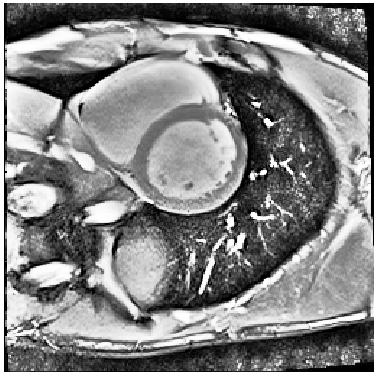
\includegraphics[width=0.19\textwidth]{./data/ohm/control/HCMNet_1100594/00_SAX/35_/im.png} &
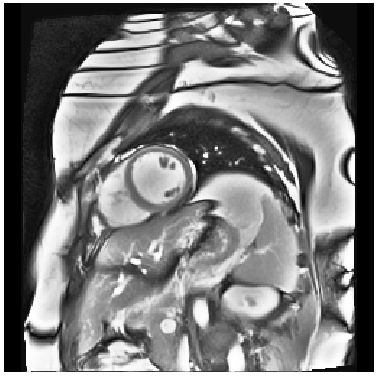
\includegraphics[width=0.19\textwidth]{./data/ohm/control/HCMNet_1100823/00_SAX/33_/im.png} &
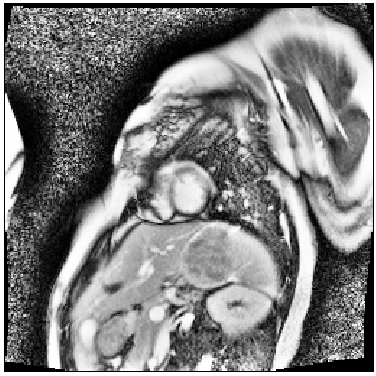
\includegraphics[width=0.19\textwidth]{./data/ohm/control/HCMNet_2600035/00_SAX/024_SA_CINE/im.png} &
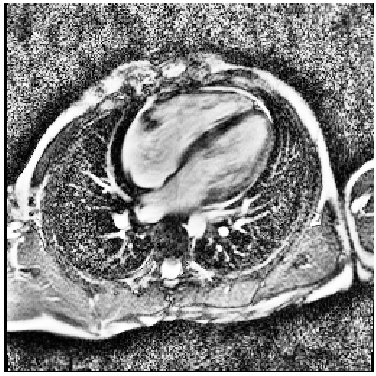
\includegraphics[width=0.19\textwidth]{./data/ohm/control/HCMNet_1700012/01_HLA/00/im.png} &
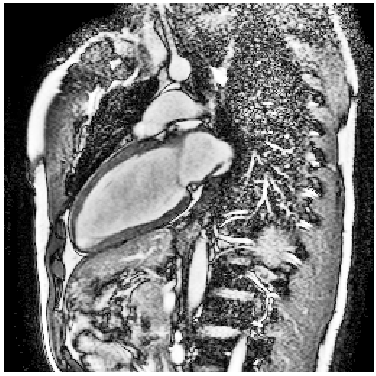
\includegraphics[width=0.19\textwidth]{./data/ohm/control/HCMNet_2100096/02_VLA/00/im.png} \\

\multicolumn{5}{c}{结构定位} \\

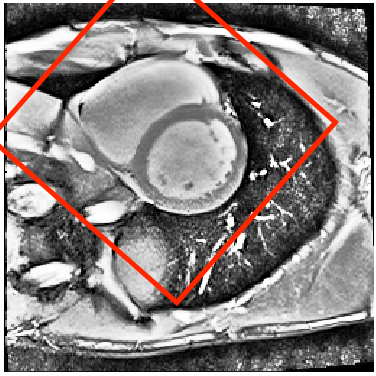
\includegraphics[width=0.19\textwidth]{./data/ohm/control/HCMNet_1100594/00_SAX/35_/im_det.png} &
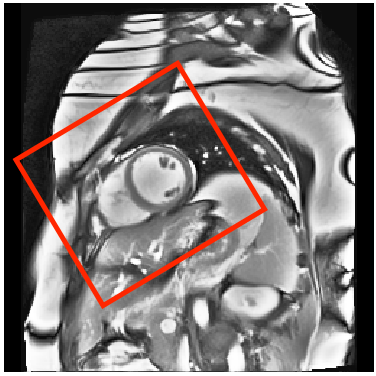
\includegraphics[width=0.19\textwidth]{./data/ohm/control/HCMNet_1100823/00_SAX/33_/im_det.png} &
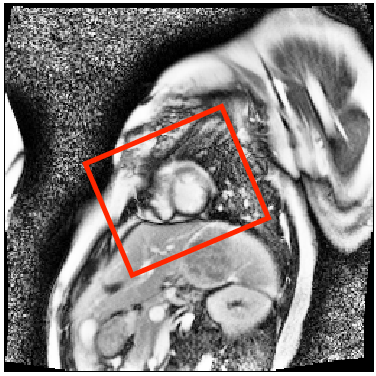
\includegraphics[width=0.19\textwidth]{./data/ohm/control/HCMNet_2600035/00_SAX/024_SA_CINE/im_det.png} &
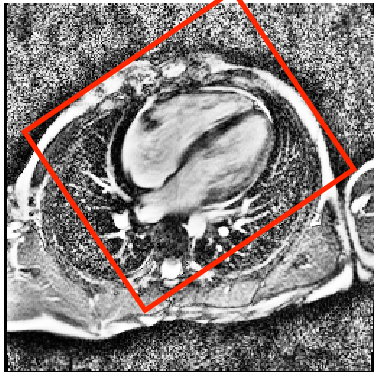
\includegraphics[width=0.19\textwidth]{./data/ohm/control/HCMNet_1700012/01_HLA/00/im_det.png} &
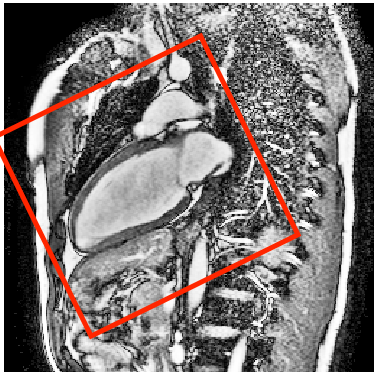
\includegraphics[width=0.19\textwidth]{./data/ohm/control/HCMNet_2100096/02_VLA/00/im_det.png} \\

\multicolumn{5}{c}{变换到典型方向的图像:$\image^\prime = \trans(\image,M)$} \\

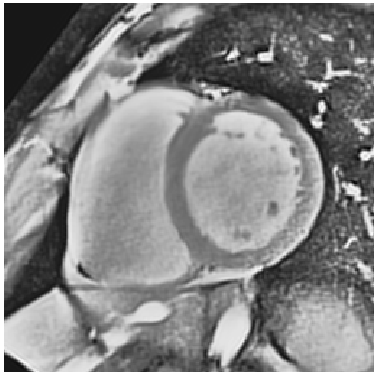
\includegraphics[width=0.19\textwidth]{./data/ohm/control/HCMNet_1100594/00_SAX/35_/im_t.png} &
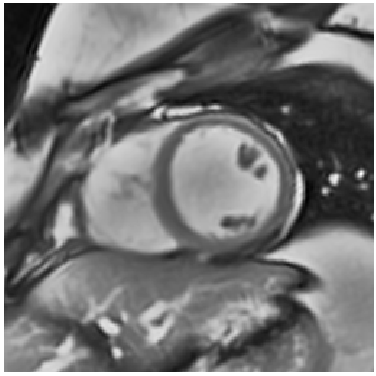
\includegraphics[width=0.19\textwidth]{./data/ohm/control/HCMNet_1100823/00_SAX/33_/im_t.png} &
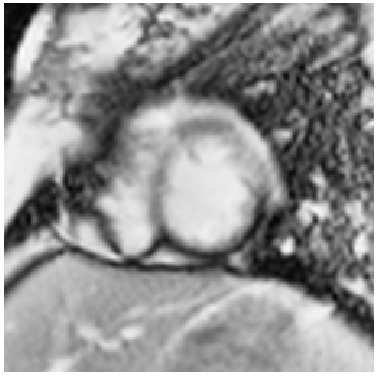
\includegraphics[width=0.19\textwidth]{./data/ohm/control/HCMNet_2600035/00_SAX/024_SA_CINE/im_t.png} &
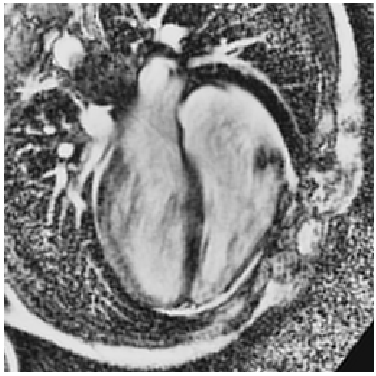
\includegraphics[width=0.19\textwidth]{./data/ohm/control/HCMNet_1700012/01_HLA/00/im_t.png} &
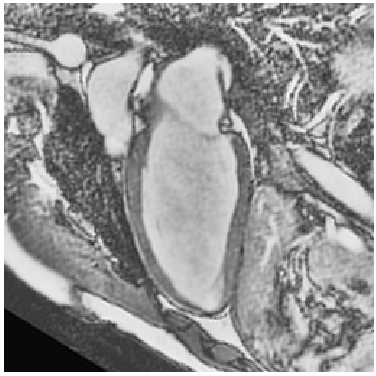
\includegraphics[width=0.19\textwidth]{./data/ohm/control/HCMNet_2100096/02_VLA/00/im_t.png} \\
\bottomrule

\end{tabular}

\caption[\captiontitle]{\captiontitle{}.
图中上面一行为短轴面(\SA{})、四腔切面(\HLA{})和两腔(\VLA{})的图像,下面一行为对应的经过一个刚体、仿射变换后变换到一个典型方向的图像.
按照临床习惯,心脏已经经过了旋转,使得 \SA{} 面的右室在放射学上的图像右侧,而左室在 \HLA{} 和 \VLA{} 面的方向是沿着长轴方向的.
心脏区域也已经移中并缩放,占到图像大小的 $90\%$.
请注意未经过方向对齐的图像中心脏的大小、方向和外观的异质,这大大增加了分割的难度.
}
\label{fig:canonical-orientation}
\end{center}
\end{figure*}
